
% !TeX root = these.tex

\chapter{Présentation de l'application}
Notre application, surnommée Betty\footnote{Brillant Ephec Time Tabling for You}, est un outil permettant d'élaborer un horaire de façon plus conviviale et plus rapide comparé à la façon actuelle de procéder à l'Ephec.\\
\newline
\indent
Cependant, avant tout développement ultérieur, il est nécessaire de présenter les différents objets composant notre solution. Nous avons choisi de travailler par \texttt{projet}. Chaque projet est caractérisé par un ensemble de cours étalés sur deux semestres. Betty permet de gérer plusieurs projets. Dans une optique de confidentialité, l'accès à chaque projet nécessite une \texttt{inscription} et une \texttt{connexion} de la part de l'utilisateur.
\newline
\indent
Au sein de chaque projet, chaque cours est représenté par ce que nous appelons un \texttt{carton}. Un carton est un cadre décrivant le nom du cours, son sigle et le professeur qui lui est rattaché. Betty propose par un système intuitif de \enquote{drag and drop} de positionner ces cartons au sein d'un \texttt{semainier} afin de construire un horaire.
\newline
\indent
Sur cette page présentant le semainier, différents outils sont utilisables afin d'améliorer la création de l'horaire. À chaque cours sont rattachés ses \texttt{attributions} spécifiques, c'est-à-dire les différentes classes d'élèves auxquelles se destine le cours. Un système de \texttt{notifications} a été mis en place afin d'offrir à l'utilisateur un retour sur les opérations qu'il effectue. Enfin, un système de \texttt{filtres} améliore la vision des données. 
\newline
\indent
La programmation par contraintes est utilisée pour définir de nouveaux horaires. Cette utilisation des possibilités s'effectue au travers d'un panneau d'\texttt{instances}. Une instance  est un état spécifique des cartons, c'est-à-dire un horaire potentiel. Lorsque l'utilisateur l'estime nécessaire, il est possible d'utiliser le  \texttt{solveur}. Le solveur est le système qui est en charge de calculer un nouvel horaire, c'est-à-dire une nouvelle instance, répondant à certaines contraintes.
\newline
\indent
Afin de diminuer les temps de chargement, un mécanisme permet d'exploiter la \texttt{mémoire cache} des navigateurs côté client. Ce procédé permet de minimiser le nombre de requêtes envoyées au serveur et améliore la rapidité de l'ensemble du système.\\
\newline
\indent
Cette présente section décrira ces différents aspects.


\section{Connexion et Inscription}

La première page de l'application propose à l'utilisateur d'entrer son nom d'utilisateur et son mot de passe. Le mot de passe est crypté en SHA-256\footnote{Secure Hash Algorithm 256 bits}, dans la base de données. La page propose également de vous inscrire via la flèche en haut à droite de la fenêtre.

\begin{figure}[!h]
	\begin{center}
	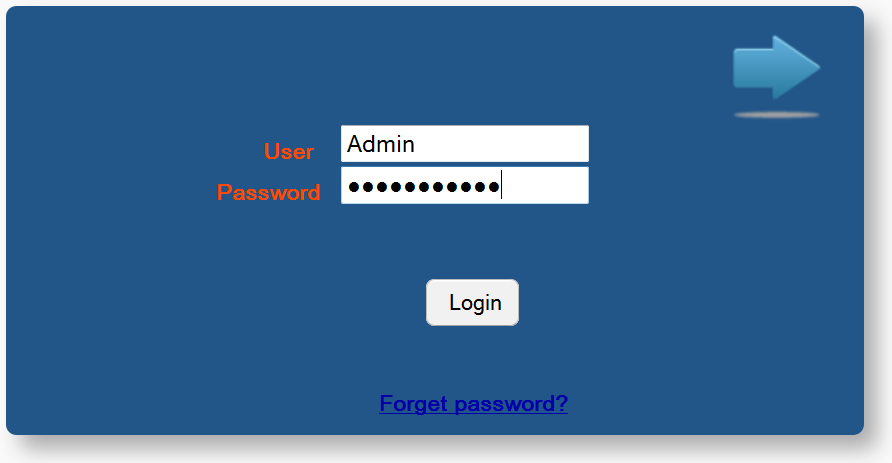
\includegraphics[width=8cm,height=4cm]{login.png}	
	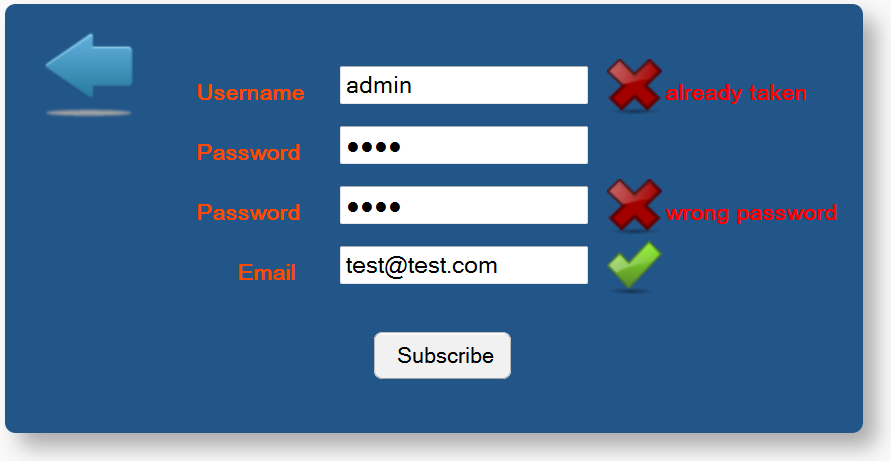
\includegraphics[width=8cm,height=4cm]{subscribe.png}
	\caption{page de login et d'inscription}
\end{center}
\end{figure}

Lors de l'inscription, nous invitons l'utilisateur à entrer sont nom d'utilisateur, mot de passe et un email. Les informations entrées sont soumises à des vérifications d'usage, le maximum de ces vérifications étant effectué du côté client afin de réduire l'échange avec le serveur.
\newline
\indent
Pour cette partie, quelques améliorations peuvent être apportées tel que le changement de mot de passe ou la récupération de celui-ci par envoi de mail.

\section{Page des projets}

La page est ordonnée de façon à avoir toujours le dernier projet en date créé en haut de la liste. Un projet est présenté de la manière la plus concise possible afin de ne pas perdre l'utilisateur. Ce dernier à la possibilité de créer un nouveau projet\footnote{Option également disponible via le menu}, choisir le semestre à élaborer et de supprimer un projet. L'application devrait dans une prochaine mise à jour proposer des options sur celui-ci tels que le partage de projets entre plusieurs utilisateurs.\\
\begin{figure}[!h]
	\begin{center}
	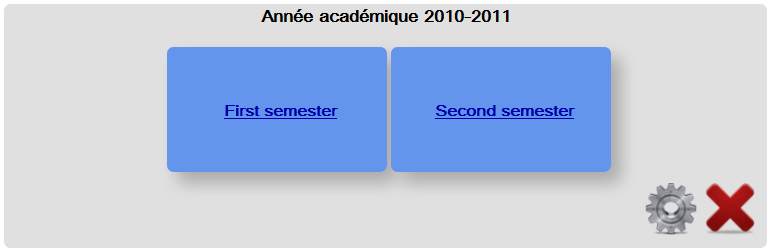
\includegraphics[width=12cm,height=4cm]{project.png}	
	\caption{représentation d'un projet}
\end{center}
\end{figure}
\\Lors de la création d'un nouveau projet, celui-ci doit être nommé et contenir les fichiers nécessaires à l'élaboration de l'horaire. Ces fichiers se présentent sous la forme d'un .xls contenant pour le premier, la liste des attributions de chaque cours, ce fichier est le résultat d'une requête SQL et nous a été fourni par l'Ephec. Le deuxième représente la liste des locaux disponibles, ce fichier n'existant pas en tant que tel, à initialement été créé par Madame Vroman, Professeur à l'Ephec, dans le cadre du "projet horaire" du cours de langage avancé de programmation de deuxième année. Nous y avons ajouté des informations pouvant être prises en compte par le solveur, et permettant de facilité l'établissement manuel d'un horaire.\\
\\
Une fois le projet créé et le quadrimestre sélectionné, l'utilisateur est redirigé vers la page principale de l'application dans laquelle l'horaire pourra être créé.

\section{Page principale}
La page principale se présente comme suit:\\

\begin{itemize}	
	
	\item Au nord de la page, nous trouvons les différents filtres et options disponibles tels que :
	\begin{enumerate}
		\item Card filter
		\item Sélection de la grille à afficher
		\item Un panneau regroupant les différentes instances du projet\\
	\end{enumerate}
	\item À l'ouest, les cartons créés sur base du fichier des attributions\\
	\item Au centre, le semainier où les cartons pourrons venir se glisser\\
	\item À l'est, un panneau de notifications permettant d'avoir un suivi des différentes actions faite par l'utilisateur.
\end{itemize}

\begin{figure}[!h]
	\begin{center}
	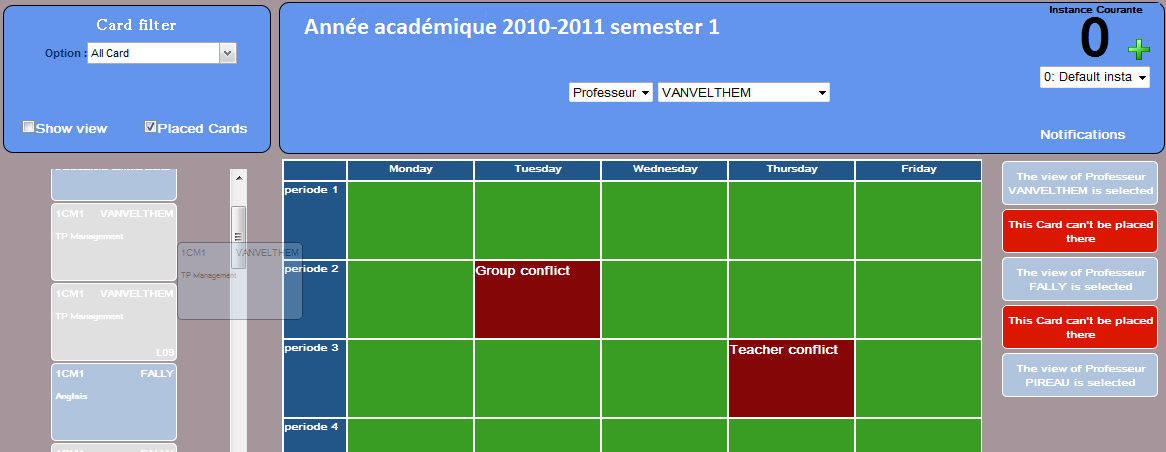
\includegraphics[width=16cm,height=6cm]{littlemain.png}	
	\caption{vue globale de la page principale}
\end{center}
\end{figure}

\subsection{Les attributions}
La mise en forme des cartons se base sur le design de ceux actuellement employés à l'Ephec lors de l'établissement manuel de l'horaire. Ceux-ci comportent le/les classe(s) assignée(s) à chaque cours donné par un professeur.\\
\newline
\indent
À chaque carton est assigné un ensemble de locaux où pourront se donner les cours. Par exemple, un carton de type informatique sera assigné uniquement aux locaux de type informatique. Lorsque le carton est déposé, la solution lui assigne un local disponible parmi cette liste, et nous pouvons voir apparaître le nom du local en bas à droite du carton.

\subsection{Semainier}
Nous affichons dans le semainier, les informations relatives à la personne, classe ou au local choisis via le filtre prévu à cet effet. La grille se colorie en fonction du carton qui est sélectionné. Un code de couleurs a été mis en place permettant de distinguer si un carton peut être placé ou pas. Par exemple, si l'on se trouve dans la vue d'une classe et que l'on prend un carton d'une autre classe, toute la grille se coloriera en rouge, montrant à l'utilisateur que celui-ci ne peut pas être placé.\\
\newline
\indent
Nous distinguons trois groupes de couleurs ; vert, orange et rouge. Ces groupes sont eux-mêmes subdivisés en trois catégories: couleur claire, normale et foncée. Lorsqu'on colorie la grille horaire, il arrive parfois qu'un carton puisse être placé à plusieurs endroits, les uns plus avantageux que d'autres pour la suite de l'établissement de l'horaire, il est donc nécessaire de pouvoir dire à l'utilisateur que le carton peut être placé, mais l'orienter sur un choix plus adéquat. Ce code de couleurs est utilisé dans une version limitée pour le moment.


\subsection{Notifications}
Les notifications sont un support pour l'utilisateur. Lorsque celui-ci effectue une action comme supprimer/ajouter un carton il est nécessaire de savoir si l'action c'est effectuée correctement. À la place d'un popup intrusif, nous avons opté pour ce système, signalant à l'utilisateur de manière plus douce l'état d'actions qui ne peuvent être vues via une interface graphique.\\
\newline
\indent
Nous distinguons ici deux couleurs différentes, une couleur se fondant au thème général de l'application lorsque tout s'est effectué correctement et une couleur rouge pour signaler un problème. Ce système est limité et pourra être amélioré dans le futur.


\subsection{Les filtres}
Les différents filtres permettent de faciliter la création de l'horaire de façon manuelle. Si nous voulons créer l'horaire d'un professeur en particulier, avoir les cartons de tous les professeurs rendrait la tâche plus lourde à l'utilisateur. L'utilisation de ce filtre permet d'avoir une meilleure vue sur ce qui doit être placé. Nous parlerons de vue \enquote{vue}.
\newline
\indent
De même, il est possible d'afficher/masquer les cartons déjà placés. Lorsqu'on filtre les cartons d'une classe et que tous ces cartons sont placés, ils ne font théoriquement plus partie de la liste des cartons et donc l'utilisateur n'a pas la possibilité de savoir si ladite classe possède des cartons. Ce système favorise aussi la vue d'ensemble sur ce qui a déjà ou non été placé.\\
\newline
\indent
Une dernière option est de pouvoir automatiquement \enquote{switcher} sur la grille horaire correspondant au filtre mis sur les cartons. Si cette option est sélectionnée et que nous filtrons les cartons de la classe \textit{3TL2}, nous supposons ici que l'objectif est de placer les attributions de cette classe. Par conséquent, seule la grille horaire des \textit{3TL2} est affichée.\\
\newline
\indent
L'application a donc été pensée afin de minimiser l'effort cognitif de l'utilisateur et de lui offrir les outils adéquats pour se concentrer sur son seul objectif ; la création de l'horaire.


\subsection{Les instances}

Le panneau d'instance permet, au sein d'un même projet, de créer un ensemble de 
sous-projets. L'objectif principal de ce panneau réside dans l'utilisation du solveur. Celui-ci sera lancé dans une nouvelle instance, permettant à l'utilisateur de continuer son horaire manuellement dans une autre sans être bloqué. Une fois la résolution finie, l'utilisateur peut naviguer entre les différentes instances afin de voir les différents résultats obtenus. \\
\newline
\indent
C'est ici que l'implémentation des instances y trouve sa principale utilité. Toutefois, il serait envisageable, comme perspective d'extension à ce travail, de pouvoir comparer deux instances entre elles.


%Cette partie est à améliorer et à modifier!
\subsection{Le solveur}
Pour lancer le solveur, nous devons aller dans le menu \texttt{project > solveur > solve}. Une fenêtre s'ouvre permettant à l'utilisateur de sélectionner l'instance dans laquelle doit s'effectuer la résolution. Une fois le solveur lancé, une notification apparaît à l'utilisateur lui notifiant que celui-ci est exécuté. À la fin de tentative de résolution, l'utilisateur reçoit une notification lui spécifiant la fin du travail et la bonne ou mauvaise application de ce dernier. Le solveur, dans sa version actuelle, fonctionne correctement, mais ne propose, à l'heure actuelle, aucune option de configuration et fonctionne sur des petits projets. 


\subsection{Mémoire cache}
L'application utilise la mémoire cache du navigateur pour stocker les données, ainsi nous minimisons les requêtes vers le serveur. Ceci pourrait être également exploité pour pouvoir travailler sur l'application sans connexion internet. Les données nécessaires à l'établissement de l'horaire étant stockées dans la partie cliente.



















